\documentclass{scrbook}

\usepackage[all]{nowidow}
\usepackage[T1]{fontenc}
\usepackage[utf8]{inputenc}
\usepackage{graphicx}
\usepackage{xcolor}
\usepackage[section]{placeins}
\usepackage{hyperref}
\usepackage{ngerman, graphicx, wrapfig, listings, float}

\definecolor{ChapterBlue}{rgb}{0.1,0.6, 0.9}
\definecolor{VerkehrsBlau}{HTML}{005A8C}
%\chapterfont{\color{ChapterBlue}}  % sets colour of chapters
%\sectionfont{\color{cyan}}
\addtokomafont{chapter}{\color{ChapterBlue}}  % sets colour of chapters
\addtokomafont{section}{\color{cyan}}
\usepackage[font={color=ChapterBlue},figurename=fig.,labelfont={bf}]{caption}

\usepackage{epstopdf}
\pagestyle{plain}
\title{Design Dokument für TODO}
\author{Christian Stricker \and Alisha Klein \and David Klopp \and Markus Vieth}
\date{\today}

\hypersetup{
	unicode = true,
	pdfborder = {0 0 0},
	linktoc = all,
	colorlinks,
	linkcolor = black,
	citecolor = black,
	filecolor = black,
	urlcolor = blue
}

\definecolor{middlegray}{rgb}{0.5,0.5,0.5}
\definecolor{lightgray}{rgb}{0.8,0.8,0.8}
\definecolor{orange}{rgb}{0.8,0.3,0.3}
\definecolor{yac}{rgb}{0.6,0.6,0.1}
\definecolor{green}{rgb}{0,.5,0}
\lstset{
	basicstyle=\scriptsize\ttfamily,
	keywordstyle=\bfseries\ttfamily\color{blue},
	stringstyle=\color{orange}\ttfamily,
	commentstyle=\color{green}\ttfamily,
	emph={@Override}, 
	emphstyle=\color{green}\texttt,
	emph={[2]Node}, %Klassen
	emphstyle={[2]\color{yac}\texttt},
	showstringspaces=false,
	flexiblecolumns=false,
	tabsize=2,
	numbers=left,
	numberstyle=\tiny,
	numberblanklines=false,
	stepnumber=1,
	numbersep=10pt,
	xleftmargin=15pt
}

\lstset{literate=
	{á}{{\'a}}1 {é}{{\'e}}1 {í}{{\'i}}1 {ó}{{\'o}}1 {ú}{{\'u}}1
	{Á}{{\'A}}1 {É}{{\'E}}1 {Í}{{\'I}}1 {Ó}{{\'O}}1 {Ú}{{\'U}}1
	{à}{{\`a}}1 {è}{{\`e}}1 {ì}{{\`i}}1 {ò}{{\`o}}1 {ù}{{\`u}}1
	{À}{{\`A}}1 {È}{{\'E}}1 {Ì}{{\`I}}1 {Ò}{{\`O}}1 {Ù}{{\`U}}1
	{ä}{{\"a}}1 {ë}{{\"e}}1 {ï}{{\"i}}1 {ö}{{\"o}}1 {ü}{{\"u}}1
	{Ä}{{\"A}}1 {Ë}{{\"E}}1 {Ï}{{\"I}}1 {Ö}{{\"O}}1 {Ü}{{\"U}}1
	{â}{{\^a}}1 {ê}{{\^e}}1 {î}{{\^i}}1 {ô}{{\^o}}1 {û}{{\^u}}1
	{Â}{{\^A}}1 {Ê}{{\^E}}1 {Î}{{\^I}}1 {Ô}{{\^O}}1 {Û}{{\^U}}1
	{œ}{{\oe}}1 {Œ}{{\OE}}1 {æ}{{\ae}}1 {Æ}{{\AE}}1 {ß}{{\ss}}1
	{ű}{{\H{u}}}1 {Ű}{{\H{U}}}1 {ő}{{\H{o}}}1 {Ő}{{\H{O}}}1
	{ç}{{\c c}}1 {Ç}{{\c C}}1 {ø}{{\o}}1 {å}{{\r a}}1 {Å}{{\r A}}1
	{€}{{\EUR}}1 {£}{{\pounds}}1
}

\begin{document}
\frontmatter
\maketitle
\tableofcontents
\mainmatter

\setcounter{part}{1}
\part{LowLevelDesign}
\chapter*{Einleitung}

In diesem Dokument wird die Implementierung unseres Systems anhand verschiedener Klassen-, sowie Sequenzdiagramme dargestellt. Hierbei wird sowohl auf die Interaktion der verschiedenen Klassen untereinander, wie auch auf die hierfür verwendeten Pattern eingegangen.\\
Das System, sowie alle Angaben zum System, beziehen sich dabei auf das ”Architectural Design Document for TODO“ vom 8. Dezember 2015.

\chapter{Apache und Tomcat}
\section{Warum Apache verwenden?}

Der Apache HTTP Server ist der meist verbreitete Webserver im Internet. 
Wir verwenden den Apache HTTP Server, da er quelloffen ist und aktiv weiterentwickelt wird. Durch diese Quelloffenheit ist der Server auf unterschiedlichen Plattformen lauffähig und leicht installier- und konfigurierbar.

 
\section{Warum Tomcat verwenden?}

Apache Tomcat ist open source und auf Grund seiner Java Implementierung ebenfalls, wie der Apache HTTP Server, plattformunabhängig. Da Tomcat die offizielle Referenzimplementierung für JavaServer Pages (JSP) und Servlets ist, ist dieser stets aktuell und wird dementsprechend aktiv weiterentwickelt. Die Implementierung der Servlets ist unabhängig von der Spezifikation des Webservers und sehr effizient, weshalb sie leicht portiert werden kann. 
Die Schnittstellen in Tomcat stellen eine klare Trennung zwischen Logik und Sicherheit bereit. Letztere wird durch die Verwendung der JavaVM weiter erhöht. 
All diese Punkte machen es leichter möglich ToDo effizient und sicher zu implementieren.   

\newpage

\chapter{Präsentationsebene}

\section{Nutzerumgebung}

\begin{figure}[h]
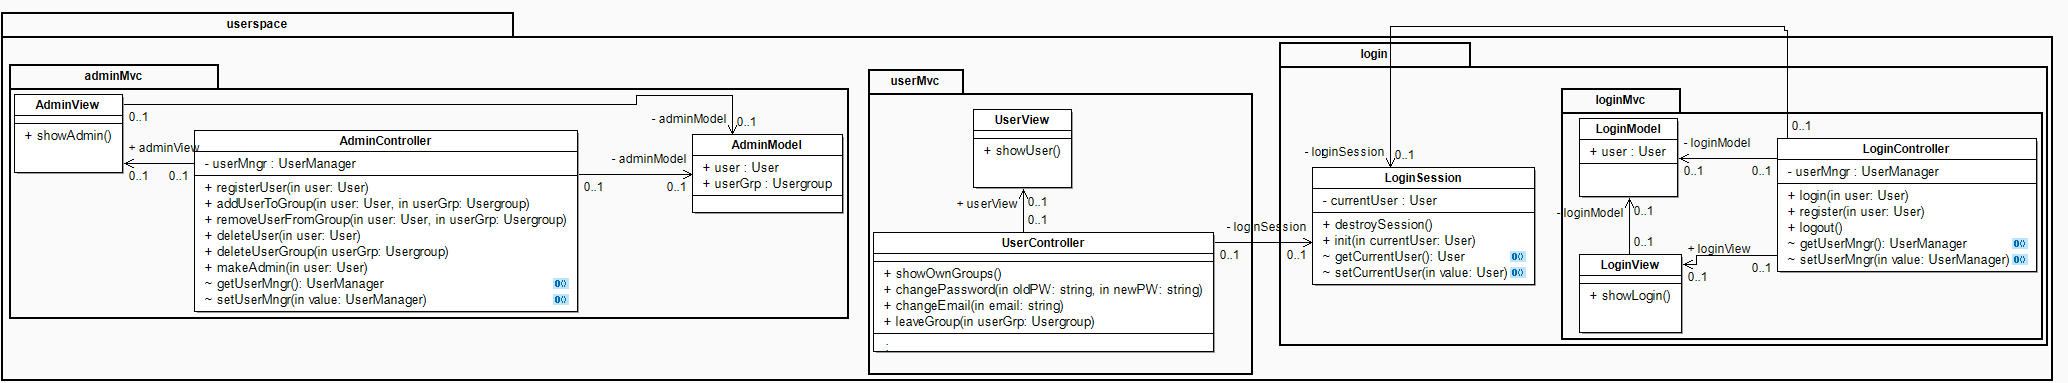
\includegraphics[width=1.0\linewidth]{Grafik/Klassendiagramme/Nutzerumgebung.png}
\end{figure}


Die Nutzerumgebung umfasst den Login-Bereich, sowie den Benutzer- und Adminbereich. Die Bereiche sind nach dem Model-View-Controller-Prinzip entworfen. Alle drei Teile werden über eine View-Klasse repräsentiert.
Weiterhin haben alle drei Bereiche jeweils einen Controller. Jeder Controller nimmt die Anfragen der entsprechenden View-Klassen entgegen und 
verarbeitet diese. Zu den Anfragen gehören im Login-Bereich anmelden oder abmelden oder neu registrieren.
Im User-Bereich kann der angemeldete Benutzer seine Angaben  ändern, sowie seine Gruppenzugehörigkeit  - soweit er die Berechtigung hat - bearbeiten.
Ein angemeldeter Administrator kann verschiedene Benutzeroperationen machen, wie Registrieren, Gruppen zuweisen, Benutzer oder -Gruppen löschen sowie  neue Administratoren benennen.
Der Adminbereich hat eine Model-Klasse, in welcher der aktuell bearbeitete Benutzer bzw. die aktuelle bearbeitete Benutzergruppe  zwischengespeichert wird.\\

\noindent Login-Bereich und User-Bereich teilen sich als Model eine Session-Klasse, welche die Informationen zum aktuell angemeldeten Benutzer hält.
\pagebreak
\section{Servlet}

% hier bitte die Grafik der Servlets
\begin{figure}[h]
\centering
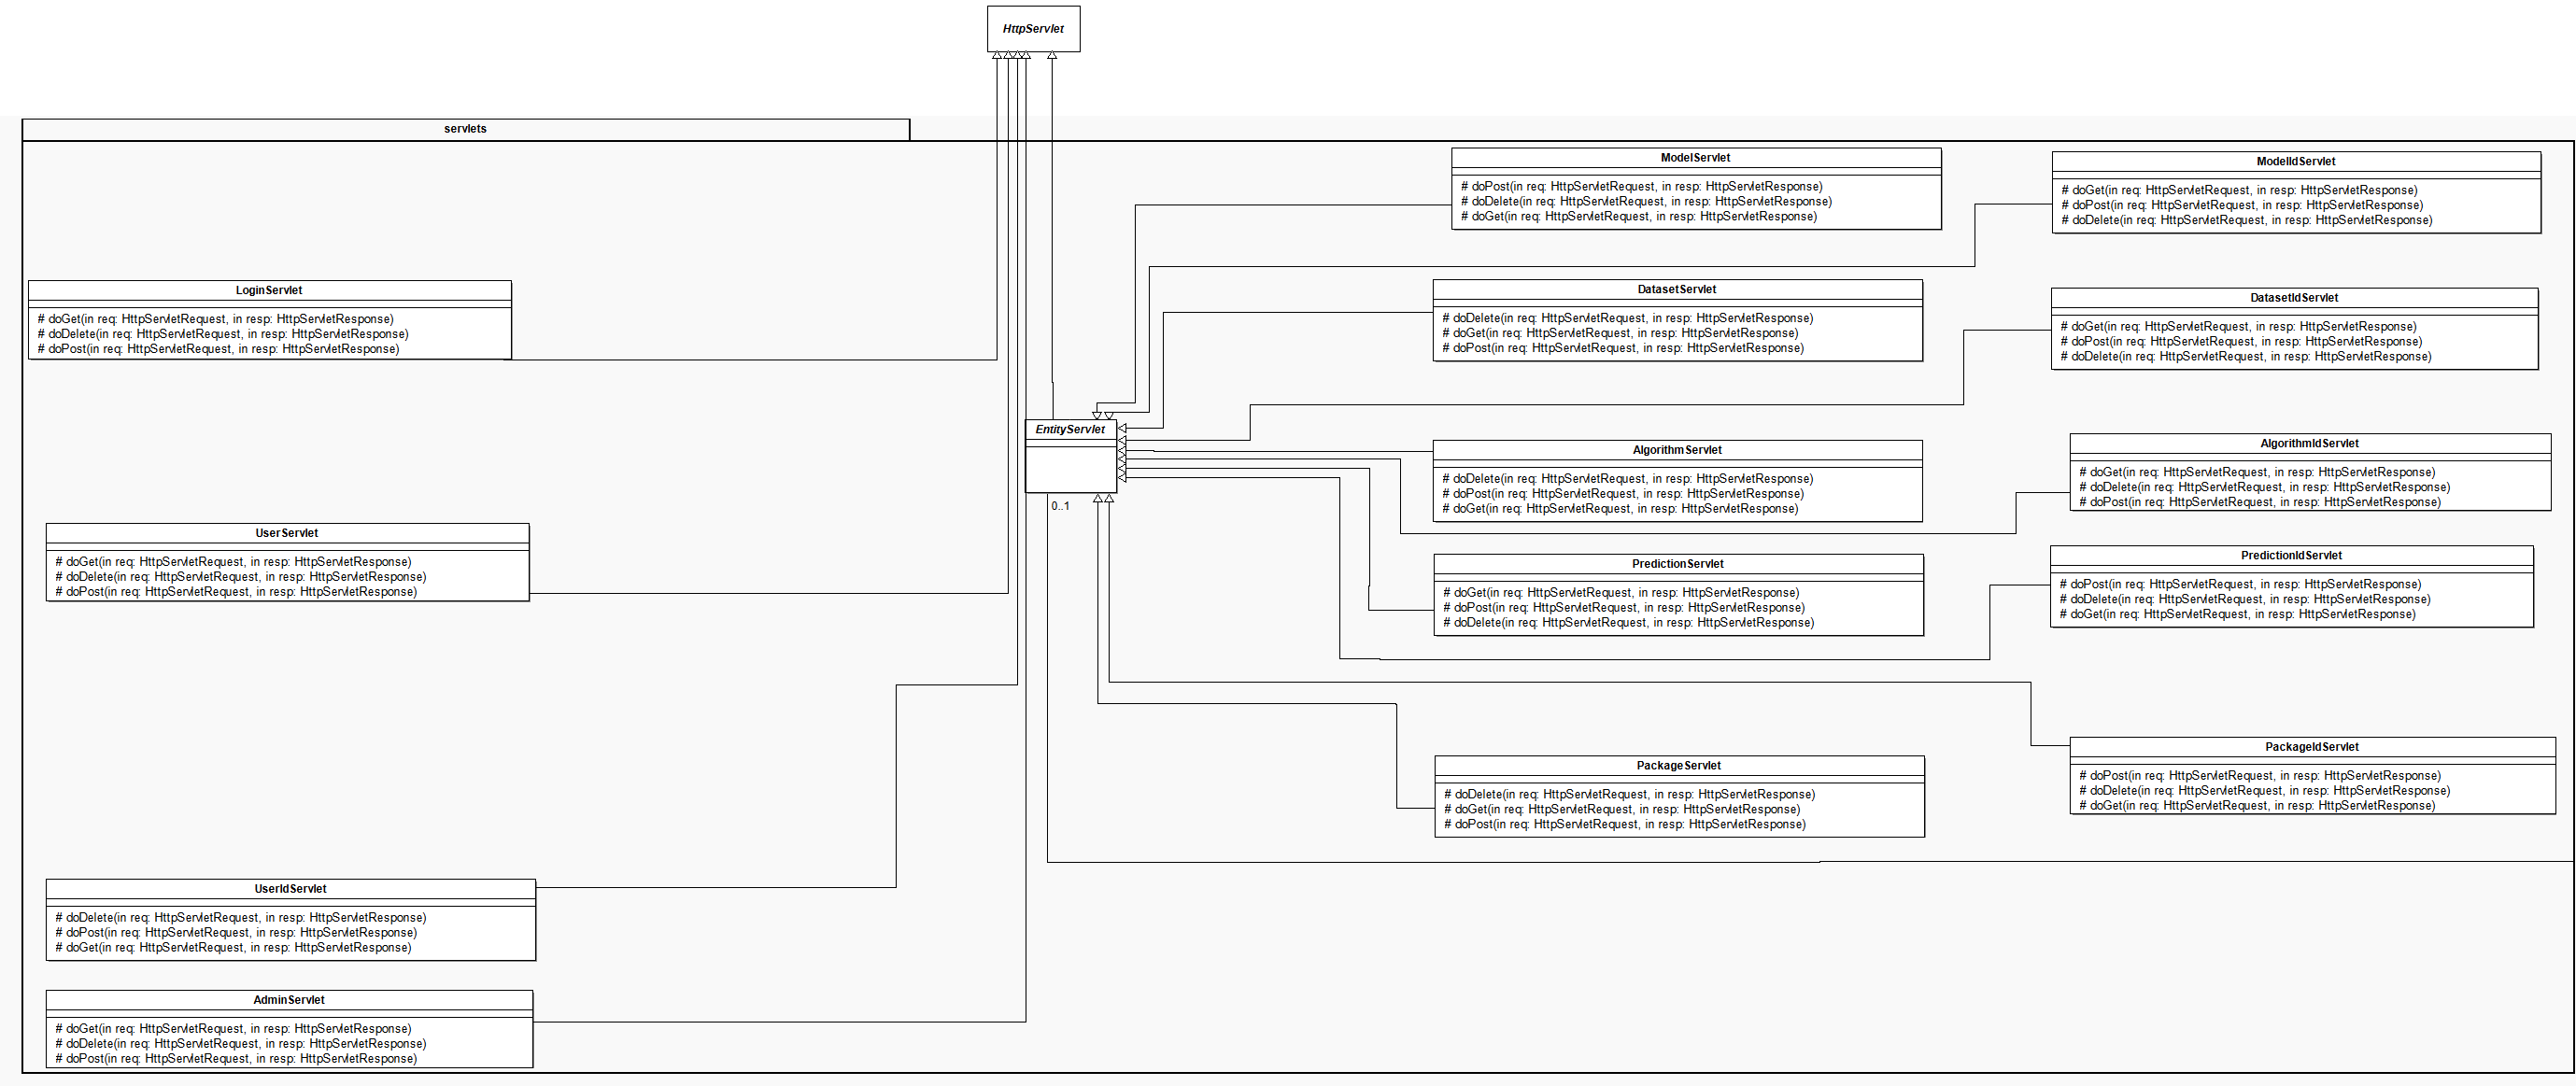
\includegraphics[width=0.9\linewidth]{Grafik/Klassendiagramme/Servlet.png}
\caption{Übersicht aller Servlets}
\end{figure}


Der Server implementiert verschiedene Servlets, die die Anfragen eines Clients entgegennehmen und beantworten. Hierzu werden die Anfragen des Nutzer ausgewertet und in der Klassenhierarchie an die zuständigen Instanzen weitergeleitet. Zu jedem REST Endpoint den das System bereitstellt existiert ein entsprechendes Servlet, welches von dem javax.servlet.http.HttpServlet abgeleitet ist. Durch diese Implementierung können leicht weitere Endpoints hinzugefügt werden, falls die nötig sein sollte. Jede Subklasse überschreit hierbei die ''doGet'' und ''doPost'' Methode, um die gewünschte Operation entsprechend der Art der Anfrage auszuführen. Hierzu kommuniziert die Servlet Klasse mit einer Subklasse des EntityControllers, der nach dem Model-View-Controller Pattern mit dem EntityModel und dem EntityView interagiert. Der EntityView realisiert hierbei den dynamischen Web-Inhalt, der dem Benutzer auf Anfrage angezeigt wird. Für jede verfügbare Ansicht existieren entsprechende Subklassen dieser drei MVC Klassen, die den jeweils benötigten Inhalt bereitstellen. 


\subsection{Abstrakte MVC-Klassen}

\begin{figure}[h]
\centering
\includegraphics[width=0.4\linewidth]{Grafik/Klassendiagramme/Entity_mvc.png}
\caption{Entity MVC}
\end{figure}

\pagebreak
\section{Entity}

\begin{figure}[h]
\centering
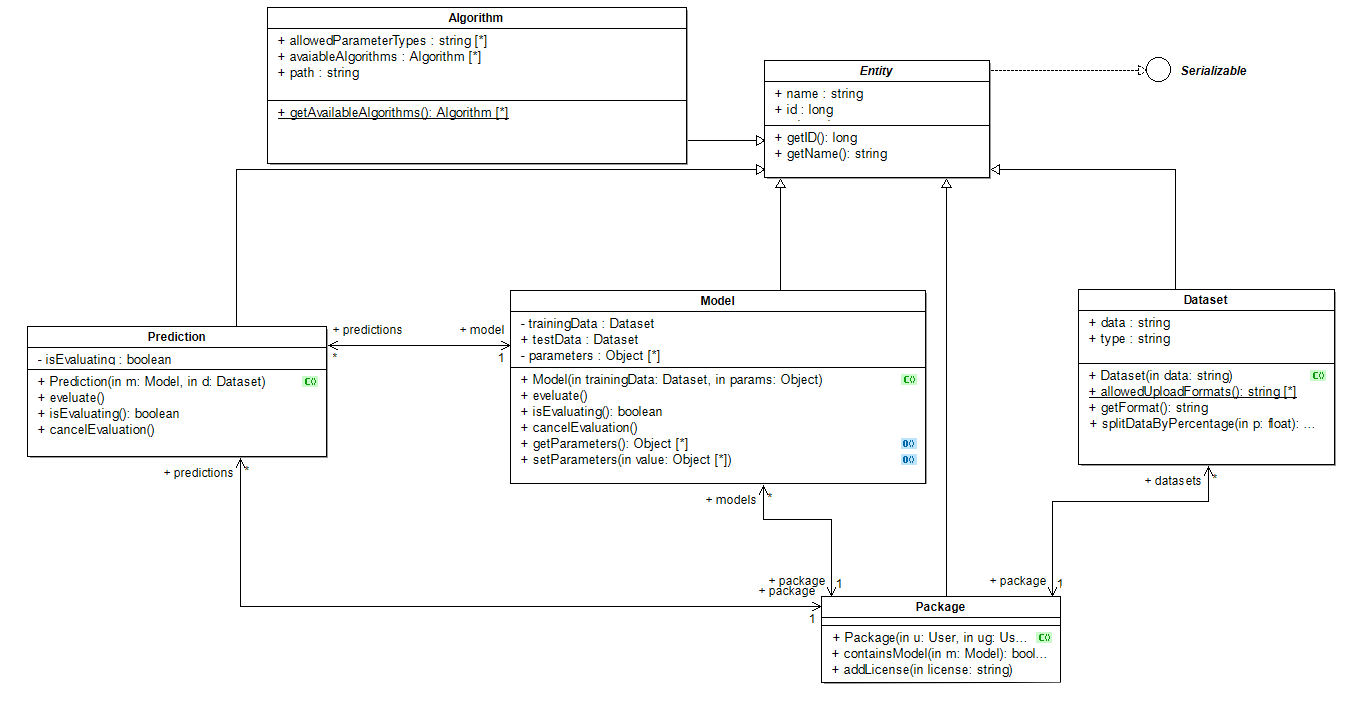
\includegraphics[width=1.0\linewidth]{Grafik/Klassendiagramme/Entity.png}
\caption{Abstrakte Superklasse}
\end{figure}

Jedes Package, Dataset, Model, jeder Algorithm und jede Prediction leiten von der Klasse Entity ab und haben somit einen eindeutige id, sowie uri und einen Namen. Über die Kommunikation mit den darüber liegenden Schichten wird der PluginLoader instruiert je nach Bedarf die jeweilig angeforderten Entities zu erzeugen bzw. abzurufen. Durch die Anbindung an die Weka-Library können die Datsets oder die Models verarbeitet werden, um so neue Predictions zu generieren.
Sämtliche administrativen Anfragen die den User oder Usergoups betreffen werden durch den UserManager gehandhabt. Dieser kooperiert über den Adapter mit dem PrivilegeManager, dem PackageManager und dem SecurityManager um die Anfragen zu beantworten.
Der Datenzugriff auf die Datenbank erfolgt vollständig über die Klasse Dataaccess, die ebenfalls an den Adapter angebunden ist. Diese Klasse bildet hierbei einen Wrapper um die SPARQL Abfragesprache um die Anfragen an die Datenbank zu formulieren und gewährleistet somit, dass keine gleichzeitigen Zugriffe auf die Datenbank erfolgen können, die zu Beschädigung führen könnten.
\pagebreak

\chapter{Logikebene}

\section{Fabrikmethode}

%@Markus: Im Zweifelsfall hau hier einfach nur die Grafik von der Fabrik rein
%... falls mir noch irgend ein halbwegs sinnvoller Text dazu einfällt ergänz ich den 
\pagebreak
\section{Adapter}

\begin{figure}[h]
\centering
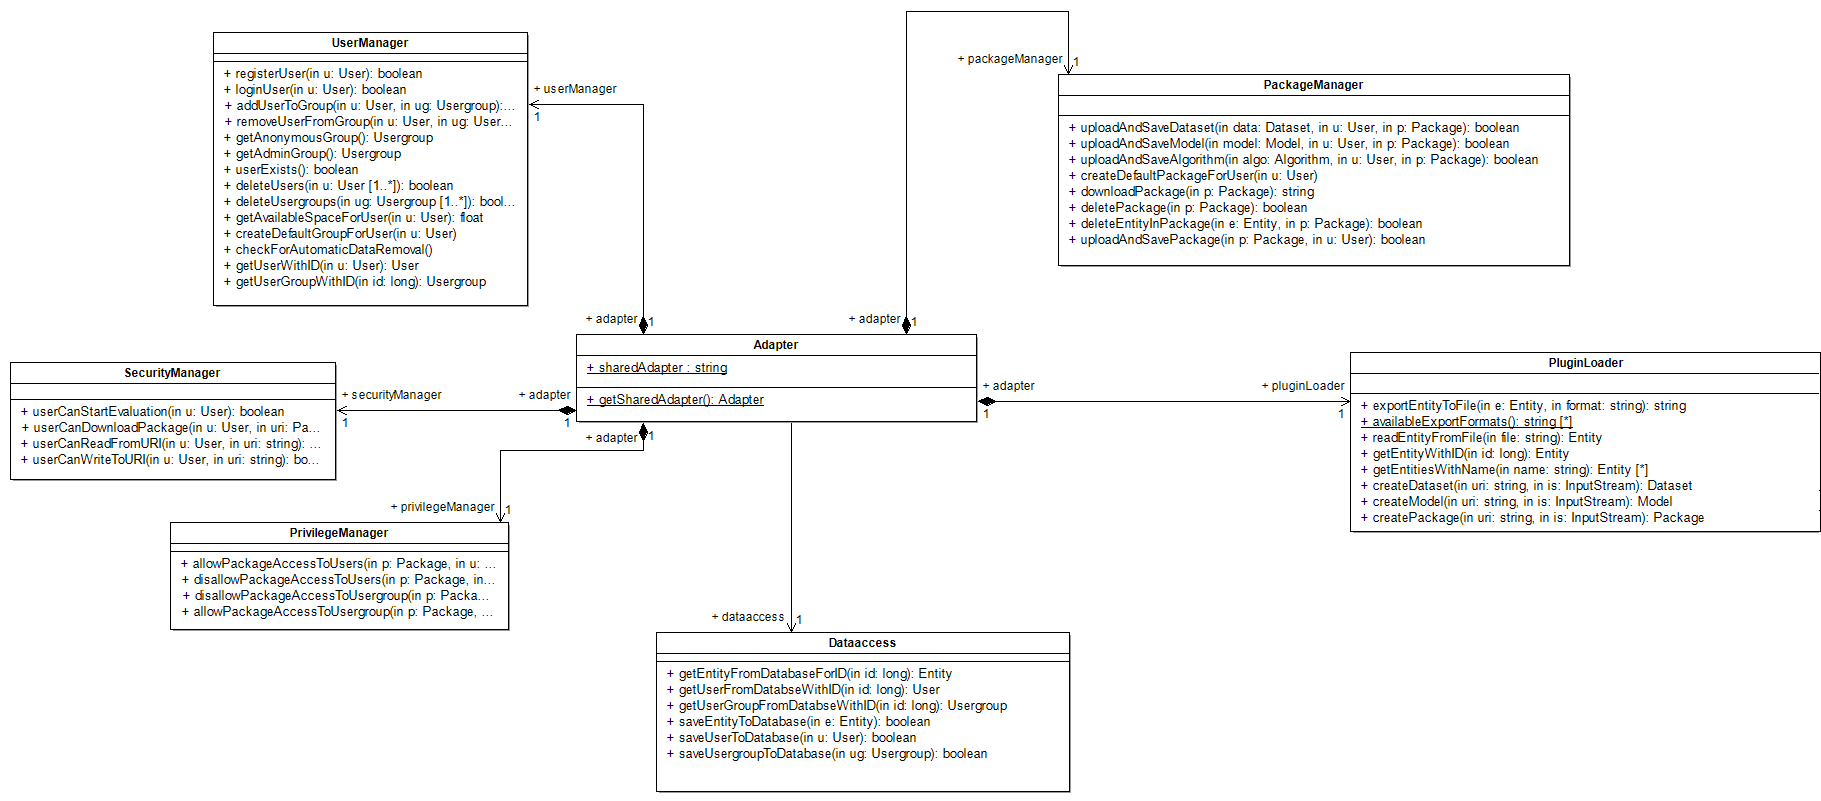
\includegraphics[width=1.0\linewidth]{Grafik/Klassendiagramme/adapter.png}
\end{figure}

Der Adapter implementiert das Singleton-Pattern, d.h. es existiert immer nur genau eine einzige Instanz der Adapterklasse. Hierbei kennt der Adapter je eine einzige Instanz der jeweiligen Kernkomponenten des Systems. Durch diese Implementierung ist ein Zugriff auf sämtliche dieser Komponenten leicht von verschiedenen Klassen aus möglich. Stellt der Nutzer beispielsweise eine Anfrage an das System, so erhalten die Klassen der Präsentationsebene über den Adapter eine Instanz der jeweils notwendigen Managerklasse, wie z.B. dem UserManager.
\pagebreak
\section{Entity}

\begin{figure}[h]
\centering
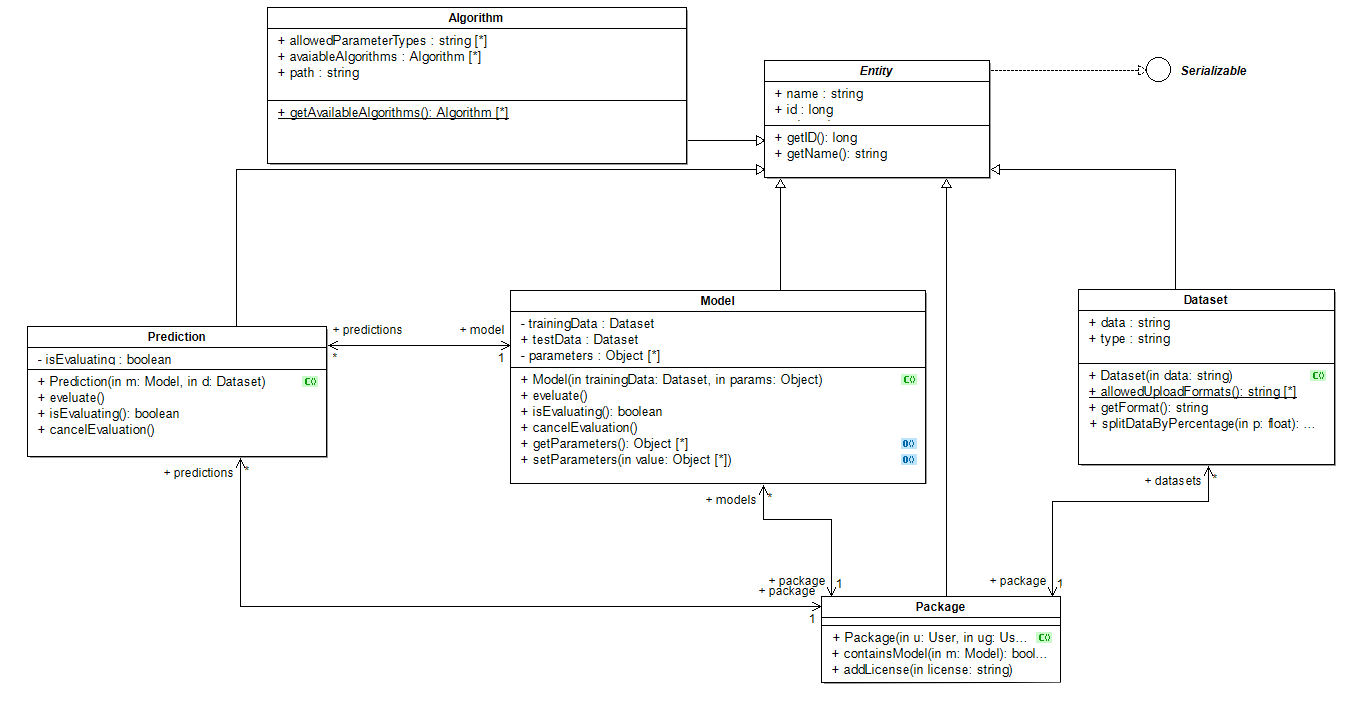
\includegraphics[width=1.0\linewidth]{Grafik/Klassendiagramme/Entity.png}
\caption{Abstrakte Superklasse}
\end{figure}

Jedes Package, Dataset, Model, jeder Algorithm und jede Prediction leiten von der Klasse Entity ab und haben somit einen eindeutige id, sowie uri und einen Namen. Über die Kommunikation mit den darüber liegenden Schichten wird der PluginLoader instruiert je nach Bedarf die jeweilig angeforderten Entities zu erzeugen bzw. abzurufen. Durch die Anbindung an die Weka-Library können die Datsets oder die Models verarbeitet werden, um so neue Predictions zu generieren.
Sämtliche administrativen Anfragen die den User oder Usergoups betreffen werden durch den UserManager gehandhabt. Dieser kooperiert über den Adapter mit dem PrivilegeManager, dem PackageManager und dem SecurityManager um die Anfragen zu beantworten.
Der Datenzugriff auf die Datenbank erfolgt vollständig über die Klasse Dataaccess, die ebenfalls an den Adapter angebunden ist. Diese Klasse bildet hierbei einen Wrapper um die SPARQL Abfragesprache um die Anfragen an die Datenbank zu formulieren und gewährleistet somit, dass keine gleichzeitigen Zugriffe auf die Datenbank erfolgen können, die zu Beschädigung führen könnten.
\pagebreak
\section{Weka}

% hier ne Grafik von unserer Weka-Klasse 


Der WekaHandler stellt einen Wrapper um die bereits bestehende Weka-Library dar. Dieser Wrapper dient dazu, die von Weka implementierten Datenstrukturen und Methoden, zu den von uns erstellten Klassen kompatibel zu machen. Der Zugriff auf sämtliche für uns relevanten Funktionen der Library kann somit einfacher erfolgen, da ein tiefgehendes Verständnis der Selbigen nur für die Implementierung des WekaHandlers erforderlich ist, nicht aber für die Verwendung der Methoden in den restlichen Klassen.

% mal schaun ob mir noch ein paar Worte dazu einfallen wenn ich die Klasse gesehen hab


\chapter{Sequenzdiagramme}
\section{Login}


\begin{figure}[h]
\centering
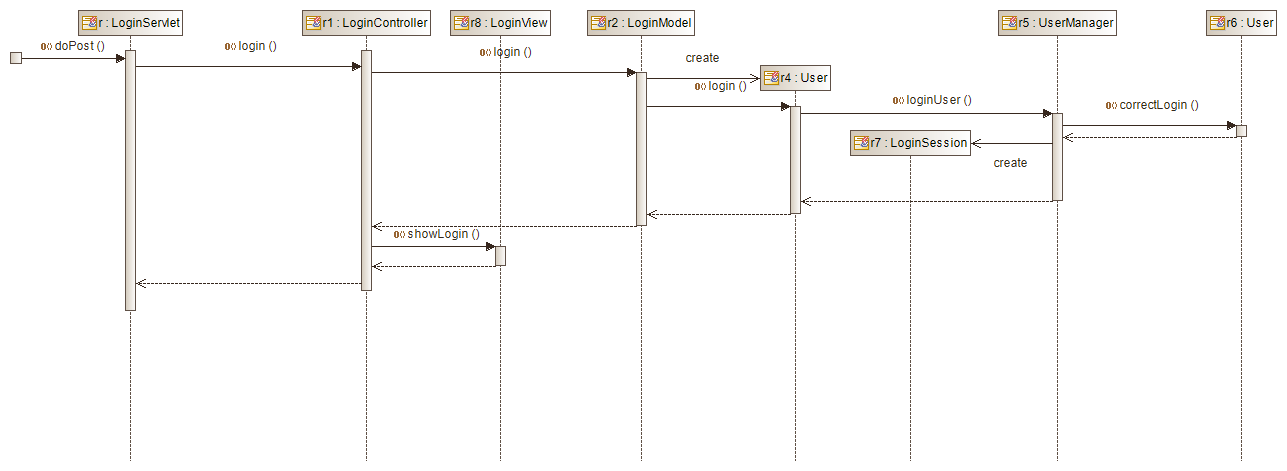
\includegraphics[width=1.0\linewidth]{Grafik/Sequenzdiagramme/Login.png}
 \caption{Login Vorgang eines Benutzers}
\end{figure}

\section{Modellerstellung}

\begin{figure}[h]
\centering
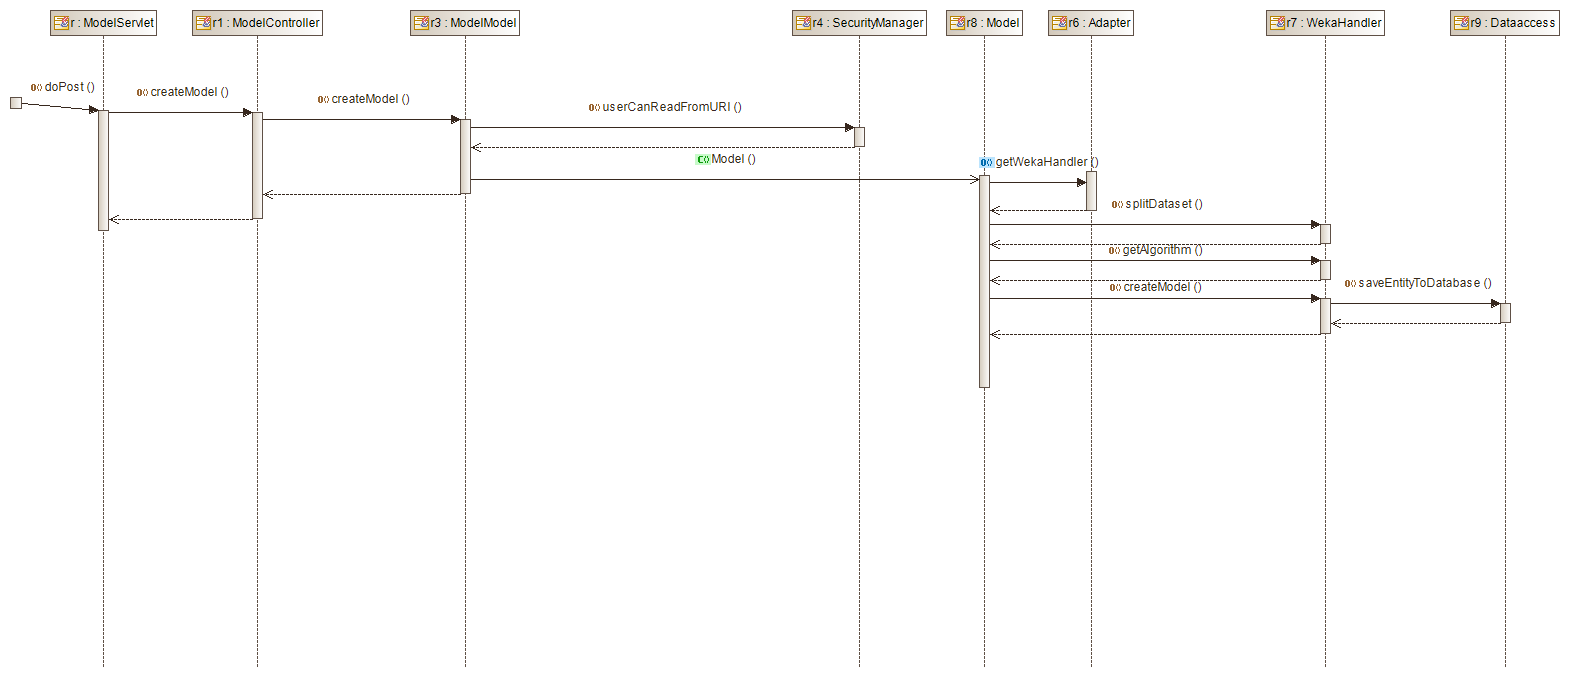
\includegraphics[width=1.0\linewidth]{Grafik/Sequenzdiagramme/Modelerstellung.png}
 \caption{Erstellung eines Modells durch den Nutzer}
\end{figure}


\end{document}
